\Chapter{Entwicklung eines Demo-Programms}

Das folgende Kapitel erläutert die Struktur, Motivation und Vorgehensweise hinter dem zu demonstrativen Zwecken entwickelten, auf dem Prozessor lauffähigen Tic-Tac-Toe Programms. Dieses vereint alle zentralen Funktionalitäten der Prozessor-Implementierung auf dem FPGA.

\Section{Struktur und Funktion des Demo-Programms}

Wie eingangs geschildert, bietet das entwickelte Demo-Programm die Möglichkeit, über die Buttons des FPGAs gegeneinander Tic-Tac-Toe zu spielen. Dabei wird mittels der Buttons BTN 0 bis BTN 3 (siehe Kapitel \ref{sec:mmuio} das Steuerkreuz über die das Spielbrett navigiert. Dabei ist das Brett zyklisch angeordnet, sodass eine Linksbewegung des Steuerkreuzes an den linken Rand dieses an die rechte Brettseite manövriert. Mittels des Buttons BTN 4 (siehe Kapitel)\ref{sec:mmuio} setzt der Zugspieler seine Markierung an der zuvor ausgewählten Position, sofern dies regelkonform ist. Das Spiel enthält keinen internen Reset und muss daher über einen Hard-Reset durch das FPGA erfolgen.

\begin{figure}[H]
	\centering
		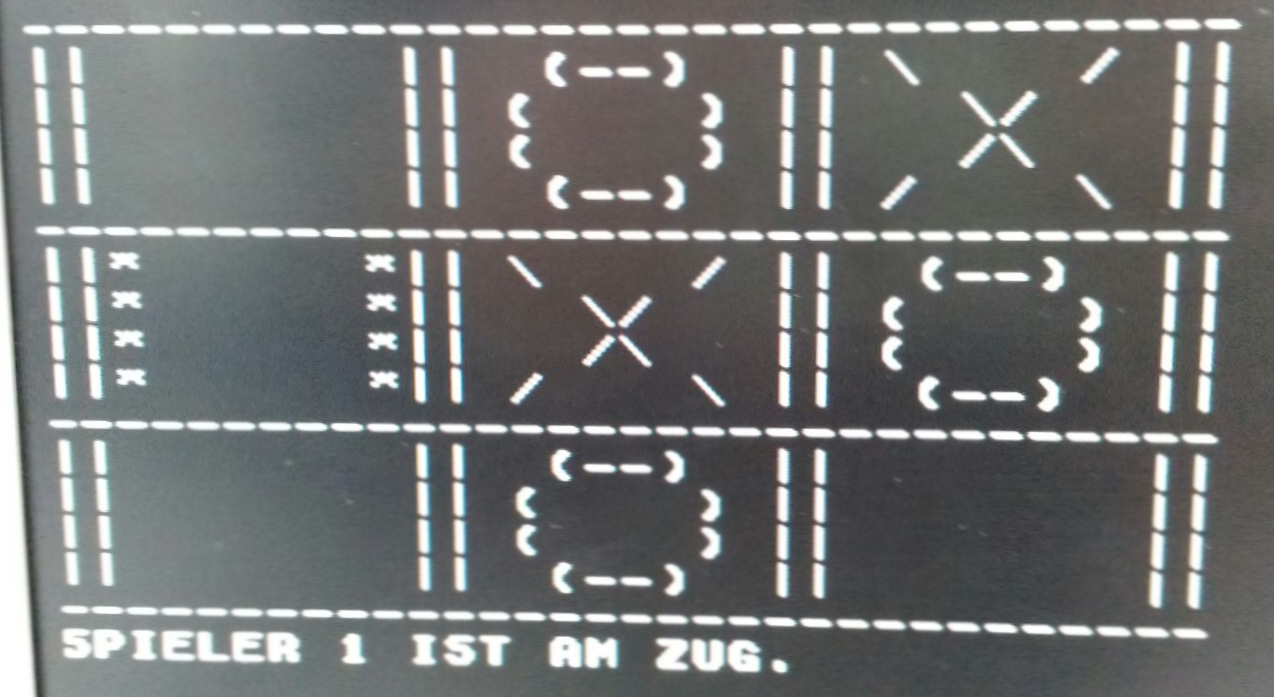
\includegraphics[width=0.5\textwidth]{gameplay.png}
	\caption{Bildschirmausgabe w\"ahrend der Ausf\"uhrung des Demo-Programms}
	\label{fig:gameplay}
\end{figure}

Um möglichst viel der implementierten Funktionalität abzudecken, wurde bei der Implementierung darauf geachtet, die meisten Komponenten zu beanspruchen. So wird bei Programmstart im DDR2-SDRAM-Block eine, als Array von vorzeichenbehafteten 8-Bit Werten realisierte, Matrix $M$ wie folgt initialisiert.

\[ M = \begin{pmatrix} -4 & -4 & -4\\ -4 & -4 & -4\\ -4 & -4 & -4  \end{pmatrix}\;
 m_{i,j} = \begin{cases}
	0 & wenn\:Markierung\:von\:Spieler\:1 \\
	1 & wenn\:Markierung\:von\:Spieler\:2 \\
	-4 & sonst

\end{cases}\]

Wobei sich anhand dieser Definition durch Spalten-, Zeilen- und Diagonalsummen sofort der Zustand des Spiels ermitteln l\"asst.

Au\ss{}erdem werden die Komponenten der grafischen Oberfl\"ache mittels Schleifen und geeigneten Subroutinen im CHARRAM(siehe \ref{tab:ramlayout}) in ihren initialen Zustand versetzt. Dabei werden zwangsl\"aufig Sprungbefehle verwendet und auf diese Weise in die Demonstration miteinbezogen.

Da der Benutzer zwangsl\"aufig mit dem Board interagieren muss, um ein Spiel zu bestreiten, nutzt das Demo-Programm auch die zuvor beschriebenen Memory-Mapped-I/O Funktionalit\"aten aus. Dazu wird, wie im folgenden Ausschnitt des Programmcodes gezeigt, in einer Endlosschleife nach neuen Eingaben auf den f\"unf verwendeten Buttons gesucht, indem durch Puffern des letzten Zustands und bitweise Verkn\"upfungen des gerade losgelassenen Buttons ermittelt wird und die Button-Nummer als R\"uckgabewert liefert. Nebeneffekte des Prellens werden hierbei allerdings nicht ber\"ucksichtigt.

\begin{lstlisting}
.key_release
	lui x26, 0x30000 //ioram prefix
	lh x27, x26, 0
	srli x27, x27, 7
	andi x27, x27, 0x1F //isolating buttons
	.key_release_wait
		//load new keys and check if any key was released
		lh x28, x26, 0
		srli x28, x28, 7
		andi x28, x28, 0x1F //new key input
		addi x30, x28, 0
		xor x28, x28, x27 //event vector (pressed and released keys)
		and x28, x28, x27 //filter released keys
		addi x27, x30, 0
		beq x28, x0, key_release_wait //keep waiting
	addi x18, x0, 0 //return value := which button was pressed
	addi x29, x0, 1
	.key_release_shift_result
		beq x28, x29, end_key_release
		srli x28, x28, 1
		addi x18, x18, 1
		jal x0, key_release_shift_result
	.end_key_release
	jalr x0, x1, 0
\end{lstlisting}

Der gesamte Programmcode umfasst circa 400 Zeilen und liegt der VHDL-Implementierung bei, wurde aber aufgrund des unverh\"altnissm\"a\ss{}igen Umfangs an dieser Stelle ausgelassen und durch den obigen Ausschnitt ersetzt.

\Section{Assemblierer und Simulator}

Aufgrund der eben erw\"ahnten Programmgr\"o\ss{}e, des reduzierten Instruction Sets und der projektspezifischen RAM-Struktur wurde der Beschluss gefasst, beim Assemblieren des Programmcodes auf einen im Rahmen des Projekts programmierten Assemblierer zur\"uckzugreifen. Auch das Debugging erfolgte durch ein eigenes Tool, welches beispielsweise Aspekte des Memory-Mapped-I/O ber\"ucksichtigen und entsprechend simulieren kann. Die beiden Programme wurden in der Scriptsprache Python entwickelt und gen\"ugen den Anspr\"uchen des Projekts insofern, als dass ein Assemblerprogramm entsprechend assembliert und simuliert werden kann, die Software allerdings keineswegs ausgiebig auf Stabilit\"at oder dergleichen getestet wurde, zumal dies nicht als Schwerpunkt f\"ur das Projekt gesetzt war.

\Subsection{Assemblierer}

Der Assemblierer ist dabei in der Lage aus einem Eingabeprogrammcode, welches Spr\"unge, Labels und Kommentare enthalten kann, einerseits Bytecode sowie eine Symboltabelle zu erstellen. Des Weiteren wird der assemblierte Programmcode auch in korrekter VHDL-Syntax ausgegeben, sodass dieser zur Initialisierung einer Dual-Port-Blockram Komponente direkt eingebunden werden kann. Dabei wird der Assemblierer als Python-Script mit den Eingabewerten als Parametern aufgerufen:

\begin{lstlisting}[language=bash]
   $ python riscv_as.py -i {input} -o {output(vhdl)} -s {symbols} file -b {binary}
\end{lstlisting}

Die Symboltabelle gibt dabei Auskunft \"uber die Speicheradresse eines im Programmcode definierten Labels. Aufgrund des modularen Aufbaus des Assemblierers k\"onnen Erweiterungen des Befehlssatzes sowie andere syntaktische Feinheiten dem Parsing- und Compilingprozess problemlos hinzugef\"ugt werden.

\Subsection{Simulator}
 
Der Simulator ist als Backend-Erweiterung zum Assemblierer gedacht, da dieser mithilfe der Ausgabedateien den Programmablauf simulieren kann. Analog zu bekannten Debugging-Umgebungen unterst\"utzt der Simulator das Setzen von Breakpoints sowie das Schrittweise Ausf\"uhren eines Befehls, w\"ahrend die verf\"ugbaren Register direkt im Blick behalten werden k\"onnen. Ferner ist es aber auch m\"oglich, den Programmablauf nach einem bestimmten Zeitintervall automatisch zu unterbrechen oder aber bestimmte Eingabesignale zu stimulieren (auch hier kann mit einem beliebigen Zeitintervall gearbeitet werden). Das Python-Script des Simulators wird in Verbindung mit dem Assemblierer wie folgt aufgerufen:

\begin{lstlisting}
   $ python riscv_as.py -i {input} -o {output(vhdl)} -s {symbols} file -b {binary}
   $ python riscv_simulation.py -s {symbols} -b {binary}
\end{lstlisting}

Dabei startet der Simulator an der Programmeinsprungsadresse und unterst\"utzt die folgenden Befehle:

\begin{table}
\begin{center}
	\begin{tabular}{| l | l |}
	\hline
		\textbf{Befehl} & \textbf{Beschreibung} \\ \hline
		n & F\"uhrt n\"achsten Befehl aus \\ \hline
		s & F\"uhrt Subroutine aus, ohne in diese zu springen\\ \hline
		c & Setzt Programmausf\"uhrung fort \\ \hline
		printchars & Zeigt die Ausgabe der ASCII-Unit\\ \hline
		bp {label/offset} & Neuer Breakpoint\\ \hline
		pin show & Zeigt alle I/O-Signale\\ \hline
		pin set {pinid} {0/1} [-d duration] & Setzt ein I/O-Signal auf einen Wert (ggf. f\"ur ein Zeitintervall in s)\\ \hline
		 m {offset} {cnt} [chunksize] & Stellt die Speicherzellen eines bestimmten Offsets blockweise dar\\ \hline
		 sleep {duration} & Unterbricht die Programmausf\"uhrung nach einem Zeitintervall in s\\ \hline 
	\end{tabular}
\end{center}
\caption{Befehls\"ubersicht des Simulators}
\end{table}

Dabei wird durch die eben beschriebenen Befehle durch die Programmausf\"uhrung navigiert, um so potenzielle Fehlerquellen zu entdecken und berichtigen. Zur Entwicklung des Demo-Programms hat der Simulator eine ma\ss{}gebliche Rolle gespielt: Nur dank dessen Funktionalit\"aten war es \"uberhaupt m\"oglich mit vertrebarem Aufwand ein vergleichsweise komplexes, funktionst\"uchtiges Programm zu entwerfen.

